\chapter{实验设计与评估}

本章旨在全面评估本文提出的面向模型推理的云边协同调度算法及 KEAS 系统的有效性。实验设计分为三个部分:核心算法仿真实验、系统功能验证实验和系统性能评估实验。首先,核心算法仿真实验重点验证分层调度优化算法的性能表现。本文通过仿真模拟了云边环境中的计算节点以及设备流式数据的生成过程,并以最关键的服务质量指标(QoS)作为评估标准,包括边缘设备调度成功率和设备请求调度成功率。实验结果定量分析了分层委托调度算法在保证设备完整调度方面的显著优势,充分体现了其在复杂云边场景下的适用性和高效性。其次,系统功能验证实验主要测试 KEAS 系统中各核心模块的功能完整性。具体而言,实验针对模型推理服务以及系统监控服务模块进行了功能性验证,确保各模块能够稳定运行并协同工作,为系统的整体性能提供可靠保障。最后,系统性能评估实验深入分析了分层调度决策对响应时间的影响,实验验证了调度算法在负载均衡方面的有效性。结果表明,分层调度策略能够根据各计算节点的实时负载状态动态分配任务,从而在不同节点间实现任务负载的合理分布。

\section{实验配置}

\subsection{仿真实验配置}

为了评估第三章提出的调度优化算法的独立效果,本文设计并实现了一个轻量级的仿真实验平台。该仿真模块基于 Python 开发,旨在模拟云边协同系统中的任务卸载决策过程。本文假设系统中包含 2 个云节点、50 个边缘节点以及 100 个终端设备。每个终端设备由一个边缘节点的设备管理器控制,其任务生成频率在 $ [1, 10] $ Hz 的范围内递增。终端设备仅负责在每个时隙开始时生成任务,而不具备本地计算能力。生成的任务需要通过调度器完成任务卸载决策,任务卸载的目标范围包括:本地边缘节点、同一边缘集群内的其他边缘节点、不同边缘集群的边缘节点以及远端的云节点。由于在工业生产场景中获取真实的工业任务数据集较为困难,本文选择通过仿真平台生成模拟任务数据,参考 KubeEdge 的数据采集方式,设备管理器根据预设的采集频率,在每个时隙开始时触发终端设备的数据采集操作。这种基于仿真的工业任务生成方式,为任务卸载决策性能的评估与优化提供了可靠的基础。表 \ref{tab:simulation-parameters} 列出了实验仿真中使用的参数设置。

% 参数设置表格
\begin{table}[ht]
    \renewcommand{\arraystretch}{1.5}
    \centering
    \caption{仿真参数设置}
    \label{tab:simulation-parameters}
    \begin{tabular}{lll}
        \toprule
        \textbf{参数} & \textbf{设置} \\
        \midrule
        终端设备数量 & 100 \\
        边缘节点数量 & 50 \\
        边缘层级数量 & 2 \\
        边缘子树数量 & 5 \\
        云端节点数量 & 5 \\
        任务数据量 & $[100 \, \text{KB}, 500 \, \text{KB}]$ \\
        边缘节点计算能力 & $2 \, \text{GHz}$ \\
        边缘节点间传输速率 & $1 \, \text{Gbps}$ \\
        边缘与云传输速率 & $128 \, \text{Mbps}$ \\
        \bottomrule
    \end{tabular}
\end{table}

为了更好地模拟工业场景中的实际需求,本文选用目标检测模型作为任务的核心计算负载。目标检测是工业界常见的应用场景之一,广泛应用于智能监控、缺陷检测和自动化流水线等领域。表 \ref{tab:model-flops} 提供了常用目标检测模型的 FLOPs 数据,用于后续分析任务计算复杂度。

% FLOPs 数据表格
\begin{table}[ht]
    \renewcommand{\arraystretch}{1.5}
    \centering
    \caption{常见目标检测模型处理单张图像的 FLOPs 数据}
    \label{tab:model-flops}
    \begin{tabular}{lll}
        \toprule
        \textbf{模型名称} & \textbf{FLOPs} \\
        \midrule
        YOLOv3\cite{redmon2018yolov3} & $65.86 \, \text{GFLOPs}$ \\
        YOLOv3-tiny & $5.58 \, \text{GFLOPs}$ \\
        YOLOv4\cite{wang2021scaled} & $109.25 \, \text{GFLOPs}$ \\
        YOLOv4-tiny\cite{gu2022novel} & $6.97 \, \text{GFLOPs}$ \\
        YOLOv5s & $16.51 \, \text{GFLOPs}$ \\
        YOLOv5-tiny & $3.49 \, \text{GFLOPs}$ \\
        \bottomrule
    \end{tabular}
\end{table}

\subsection{系统实验配置}

本实验环境基于两台 X86 架构的物理服务器和一台配备 NVIDIA RTX 3080 GPU 的高性能服务器构建。其中,配备 RTX 3080 GPU 的服务器充当云端节点。每台物理服务器上部署了 libvirt 虚拟化管理平台,通过QEMU/KVM技术构建跨主机虚拟机集群,从而实现异构计算资源的统一调度与高效管理。为了模拟真实的云边协同场景,本文利用 Open vSwitch 创建虚拟网卡,并在路由器上配置相关路由规则,从而实现虚拟机之间的互联互通。通过限制虚拟网络接口的带宽和延迟,本文能够精确模拟不同网络条件下的云边通信环境。实验环境的整体架构如图\ref{fig:5-1all}所示。

\begin{figure}[ht]
  \centering
  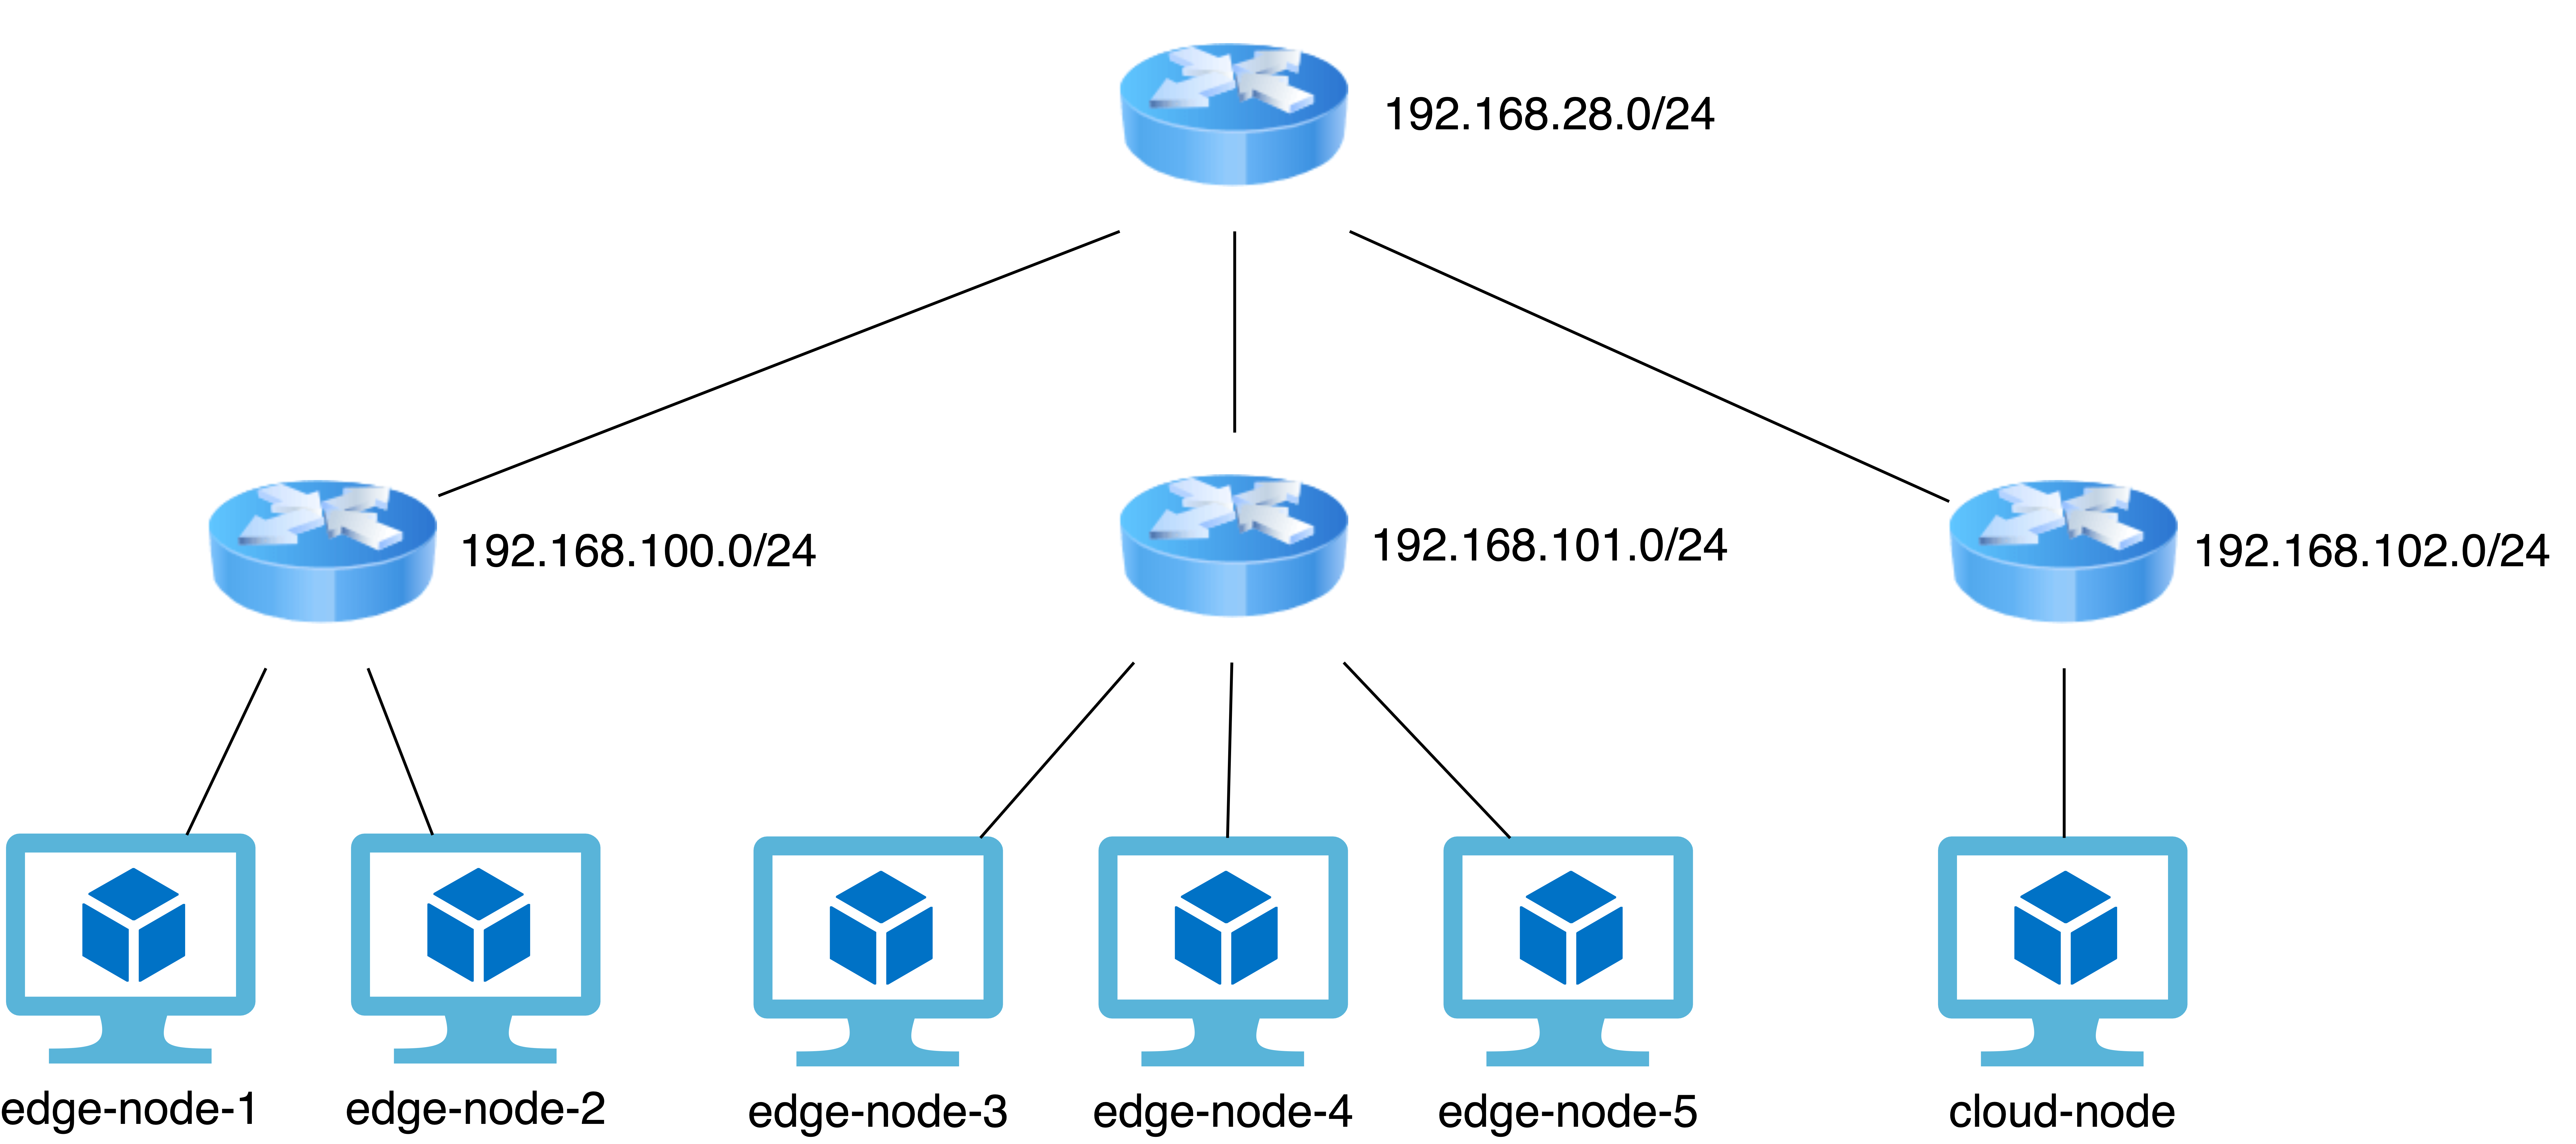
\includegraphics[width=\linewidth]{pics/5-1all.png}
  \caption{系统实验环境网络拓扑图}
  \label{fig:5-1all}
\end{figure}

具体配置参数如表\ref{tab:vm-configurations}所示。

\begin{table}[ht]
    \centering
    \renewcommand{\arraystretch}{1.2}
    \caption{实验环境虚拟化节点配置}
    \label{tab:vm-configurations}
    \begin{tabular}{cccccccc}
        \toprule
        \textbf{序号} & \textbf{设备名称} & \textbf{CPU} & \textbf{内存} & \textbf{系统} & \textbf{架构} & \textbf{IP地址} & \textbf{子网掩码} \\
        \midrule
        1 & edge-node-1 & 2核 & 4GB & Ubuntu 22.04 & amd64 & 192.168.100.1 & 255.255.255.0 \\
        2 & edge-node-2 & 4核 & 8GB & Ubuntu 22.04 & amd64 & 192.168.100.2 & 255.255.255.0 \\
        3 & edge-node-3 & 2核 & 4GB & Ubuntu 22.04 & amd64 & 192.168.101.1 & 255.255.255.0 \\
        4 & edge-node-4 & 2核 & 4GB & Ubuntu 22.04 & arm32 & 192.168.101.2 & 255.255.255.0 \\
        5 & edge-node-5 & 2核 & 4GB & Ubuntu 22.04 & arm64 & 192.168.101.3 & 255.255.255.0 \\
        6 & cloud-node & 8核 & 32GB & Ubuntu 22.04 & amd64 & 192.168.102.1 & 255.255.255.0 \\
        \bottomrule
    \end{tabular}
    \vspace{6pt}
\end{table}

本文的系统实验基于 KubeEdge 搭建,并选择目标检测作为核心任务负载,以评估调度算法在实际工业场景中的性能表现。为了生成目标检测任务所需的数据流,本文在 Ubuntu 系统上创建了虚拟的 USB 摄像头设备。具体而言,本文利用 Linux 内核模块 \texttt{v4l2loopback} 创建虚拟视频设备,该模块能够模拟真实的摄像头输入,并支持多种分辨率和帧率设置,从而为实验提供多样化且可控的数据源。进一步地,通过 FFmpeg 工具生成合成视频流并将其绑定到虚拟视频设备,确保数据流的稳定性与一致性。此外,借助 KubeEdge 的设备管理接口 DMI,动态调整虚拟设备的采集频率和数据大小,灵活配置实验参数。图 \ref{fig:dmi-config} 展示了部分 DeviceModel 配置文件。

\begin{figure}[ht]
    \centering
    \begin{lstlisting}[
        language=YAML,
        basicstyle=\small\ttfamily, 
        numbers=left, % 可选:添加行号
        numberstyle=\tiny\color{gray}, % 可选:行号样式
        frame=shadowbox
    ]
apiVersion: devices.kubeedge.io/v1beta1
kind: DeviceModel
metadata:
  name: camera-usb
  namespace: default
spec:
  protocol: camera-usb
  properties:
    - name: Framerate
      description: Framerate
      type: FLOAT
      accessMode: ReadWrite
    - name: Brightness
      description: Brightness
      type: INT
      accessMode: ReadWrite
      maximum: "127"
      minimum: "-127"
    - name: Contrast
      description: Contrast
      type: INT
      accessMode: ReadWrite
      maximum: "511"
      minimum: "0"
    ...
\end{lstlisting}
    \caption{USB 摄像头设备管理器部分配置文件}
    \label{fig:dmi-config}
\end{figure}

\section{核心算法仿真实验}

\subsection{调度优化算法比较}

本文将提出的分层调度优化算法与以下基准算法进行对比分析,这些算法在工业界中具有一定的代表性,具体描述如下:

\begin{enumerate}
    \item \textbf{全部本地执行算法(All Local Execution,ALE)}:所有的设备流式数据都在本地执行,不需要卸载。
    \item \textbf{随机卸载算法(Random Offloading Algorithm,ROA)}:该算法通过随机选择卸载目标节点来分配任务。
    \item \textbf{轮询卸载算法(Round-Robin Algorithm,RRA)}:该算法按照固定的顺序依次分配任务到不同的边缘或云端节点。
\end{enumerate}

本文最大的服务质量(QoS)指标是边缘设备调度成功率和设备请求调度成功率,其中边缘设备调度成功率指边缘设备生成的流式数据能够被完整处理的比例,该指标反映了系统对边缘设备任务的整体处理能力;设备请求调度成功率指设备生成的流式数据中成功被处理的比例,该指标更关注单个任务请求的完成情况,尤其是在高负载场景下的表现。

本文通过对比实验对于 EdgeMesh 网关提供的轮询卸载和随机卸载方法,在高请求率场景下表现出明显的性能不足。具体而言,当任务到达率超过系统处理能力时,这两种方法往往会出现显著的丢包现象和响应延迟增加的问题。随机卸载算法由于缺乏对节点负载状态的感知,随机选择卸载目标可能导致部分节点过载,而其他节点资源闲置,从而降低整体调度效率。轮询卸载算法尽管通过固定顺序分配任务能够在一定程度上平衡负载,但其静态调度策略无法适应动态变化的网络环境和突发流量,导致在高请求率下性能急剧下降。

\begin{figure}[ht]
    \centering
    \begin{subfigure}{\textwidth}
        \centering
        \begin{subfigure}{0.48\textwidth}
            \centering
            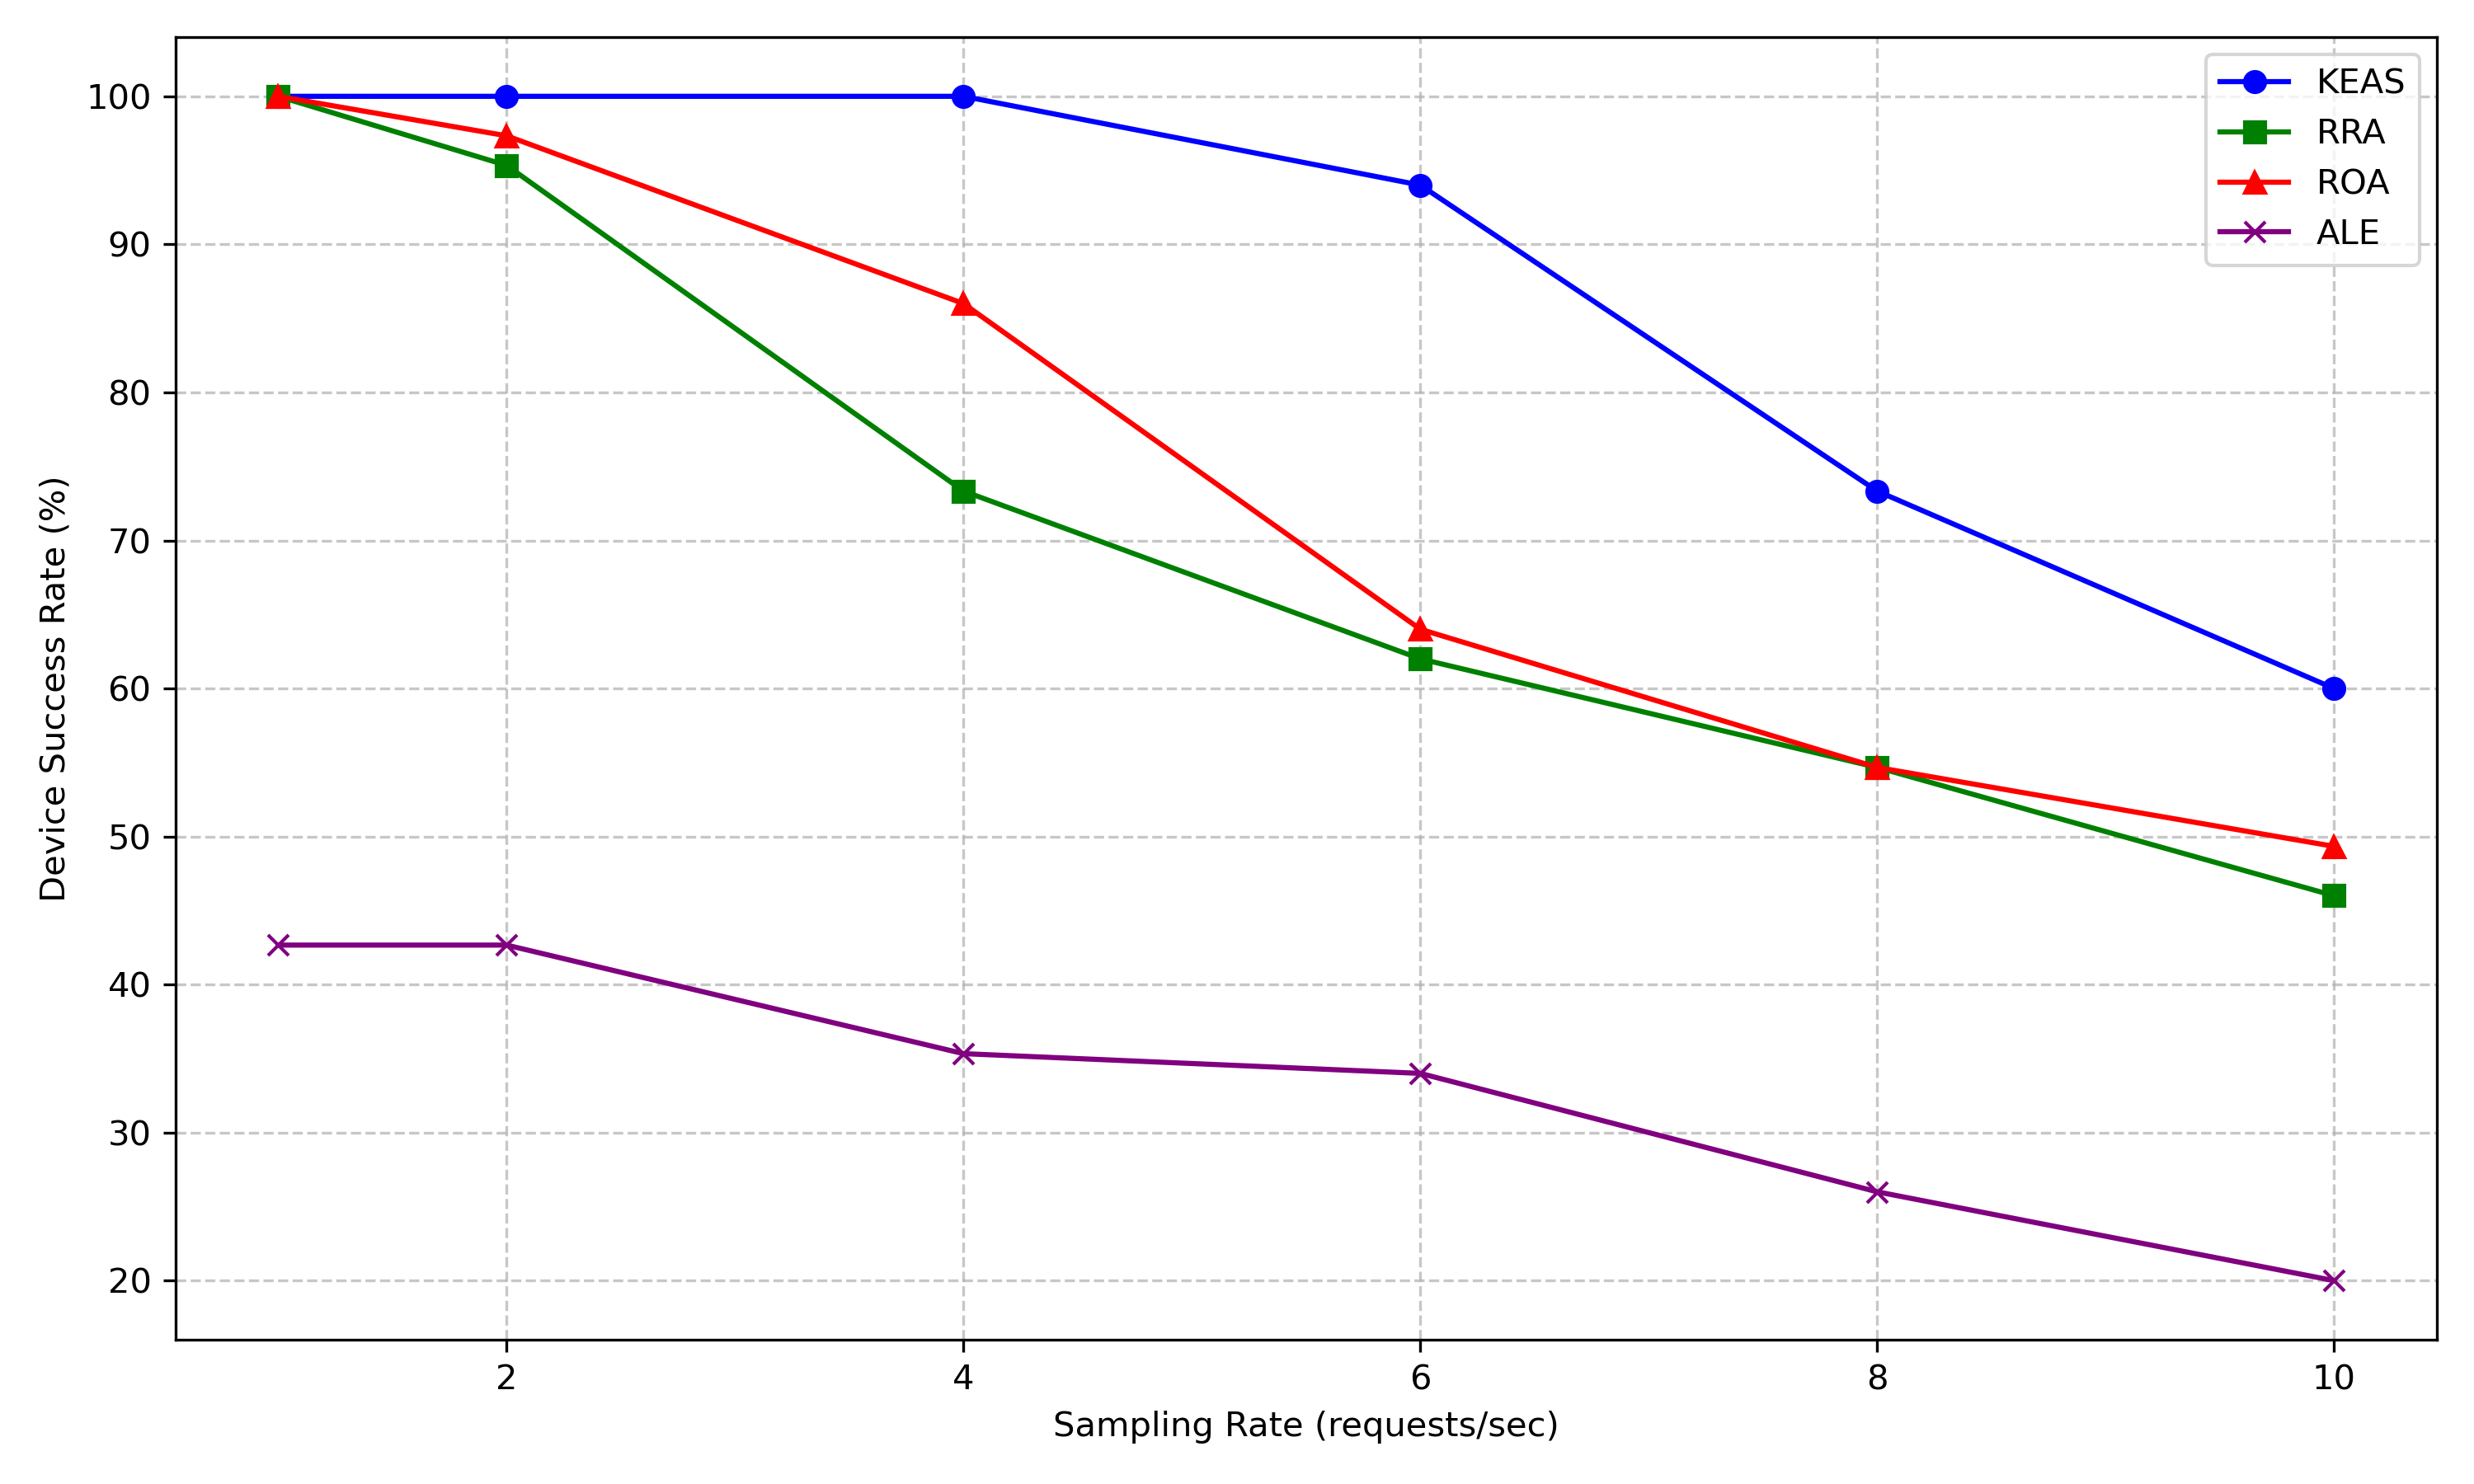
\includegraphics[width=\linewidth]{pics/expr/exp9_device_success_rate.png}
            \caption{边缘设备调度成功率}
            \vspace{0.3cm}
        \end{subfigure}
        \begin{subfigure}{0.48\textwidth}
            \centering
            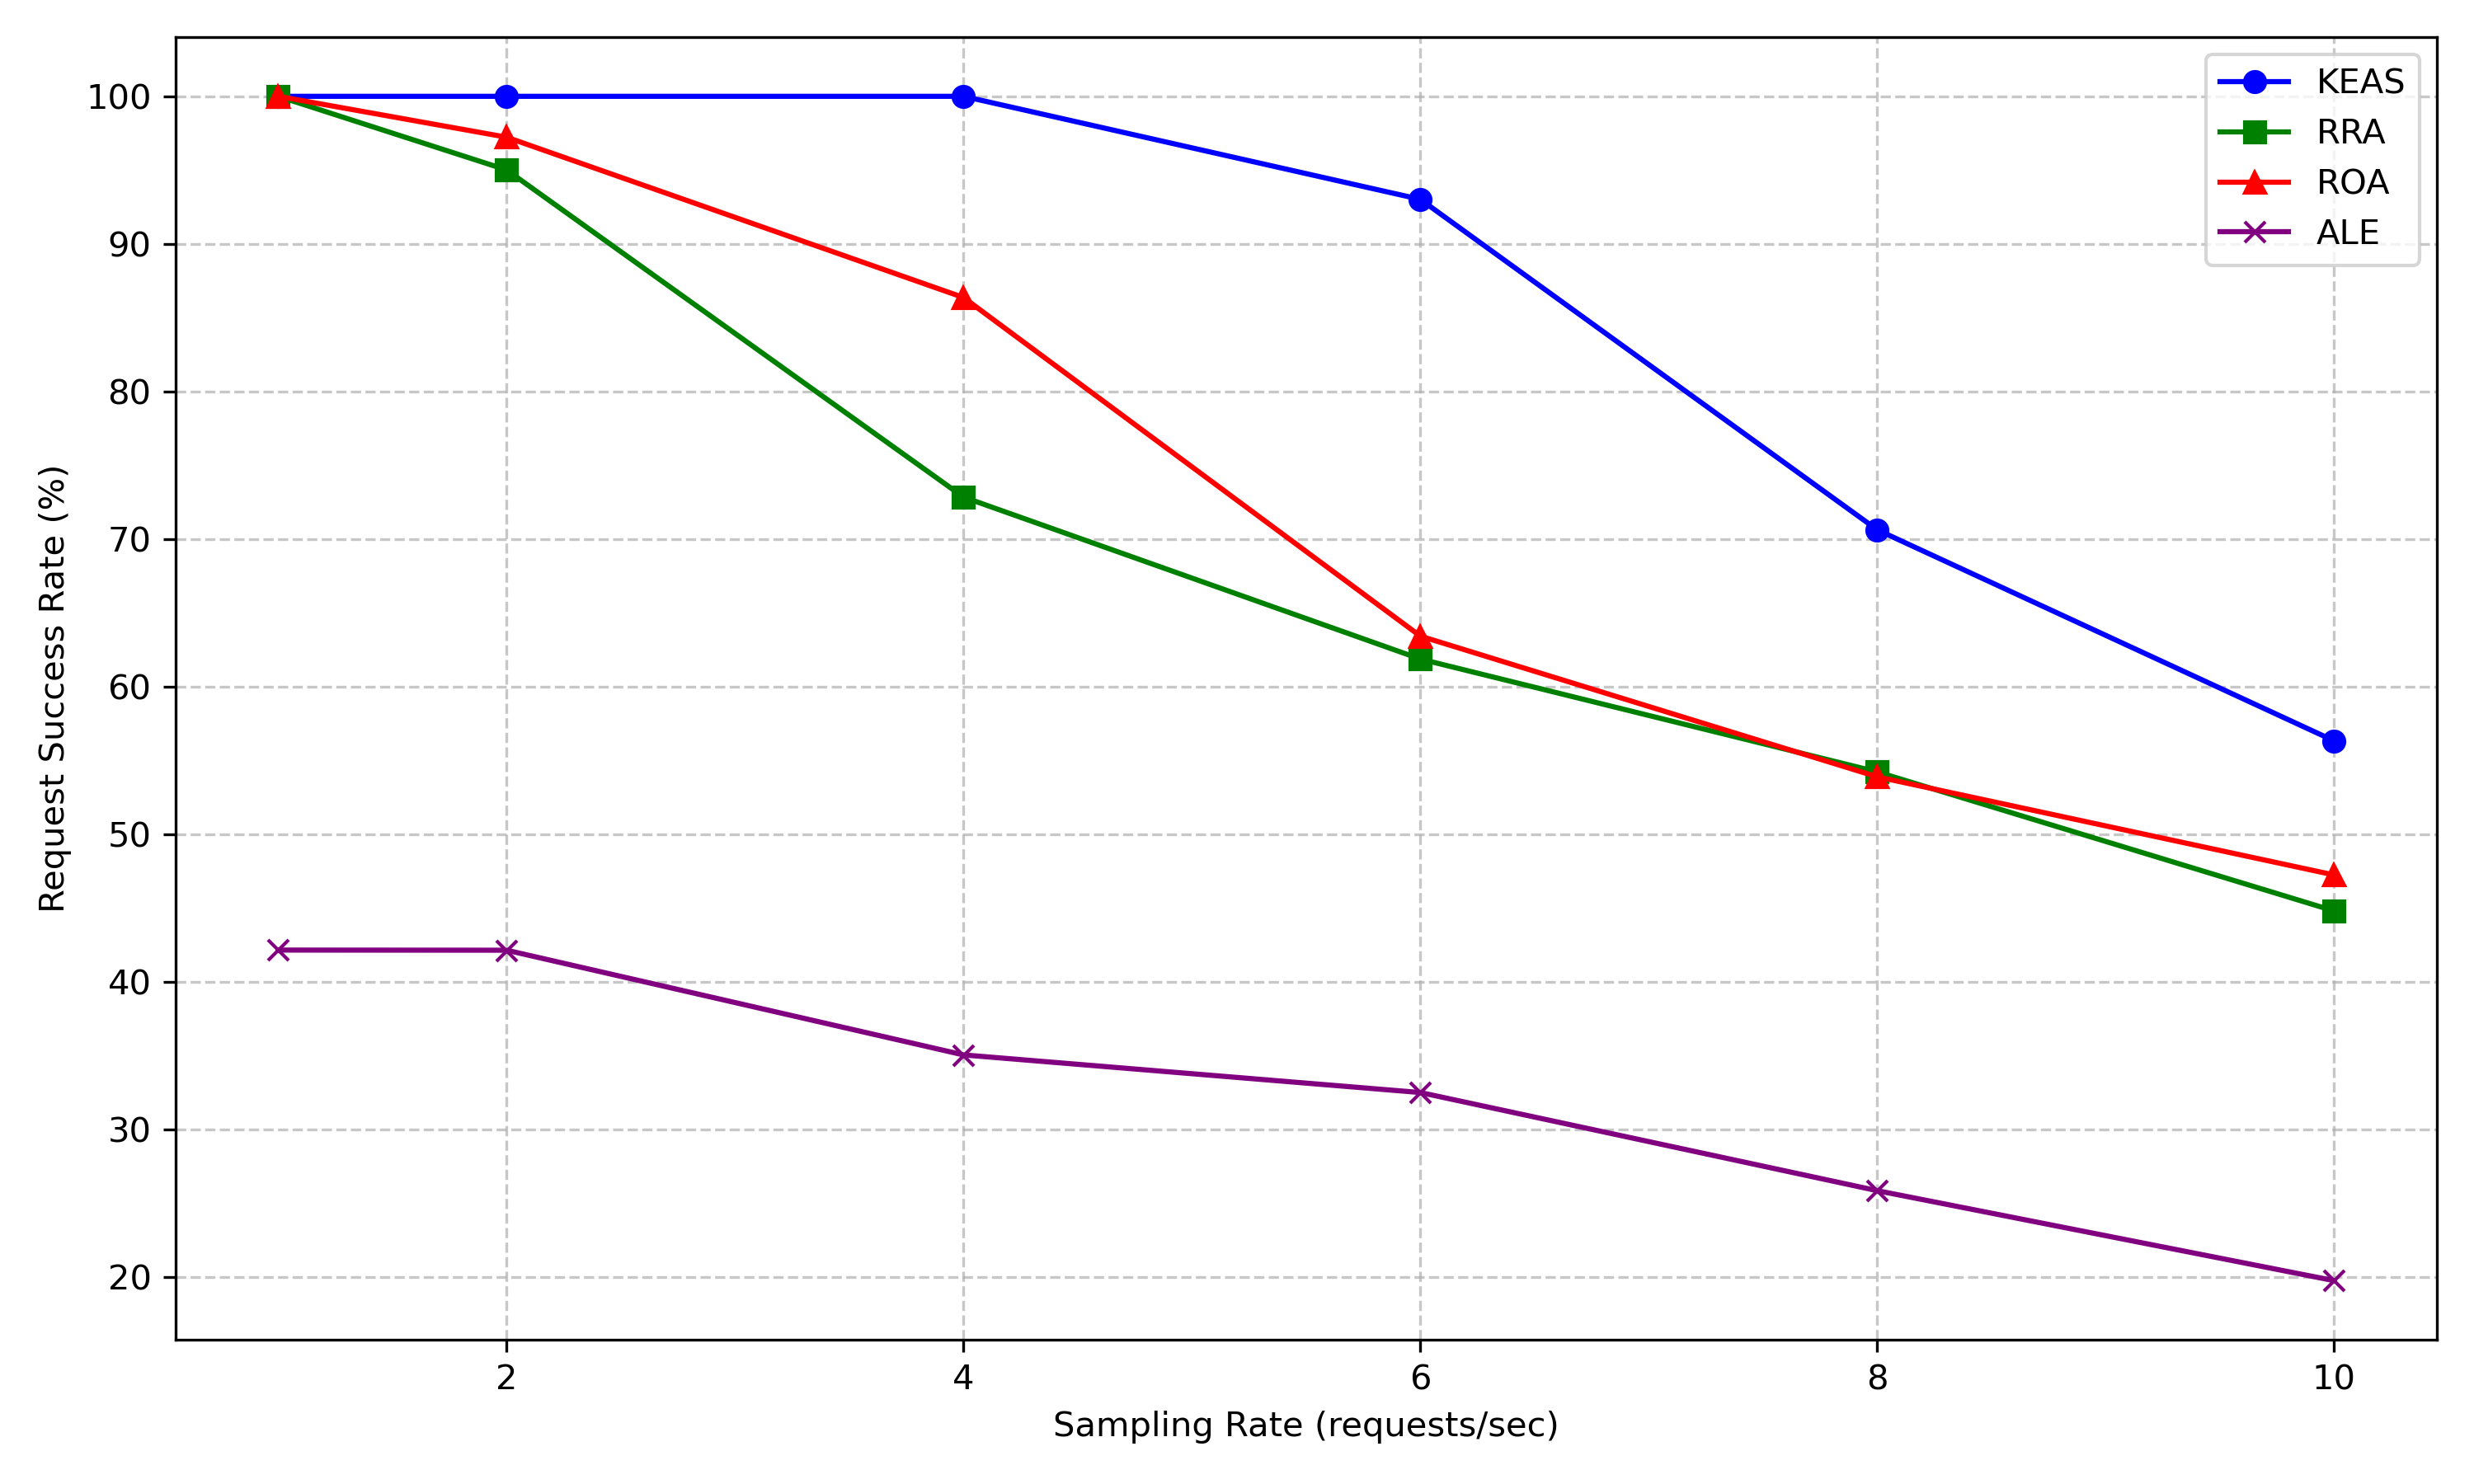
\includegraphics[width=\linewidth]{pics/expr/exp9_request_success_rate.png}
            \caption{设备请求调度成功率}
            \vspace{0.3cm}
        \end{subfigure}
    \end{subfigure}
    \caption{不同调度策略的服务质量对比}
    \label{fig:exp1}
\end{figure}

\subsection{分层调度器实验分析}

本文针对每一层级的调度设计了相应的优化算法,这些算法分别针对不同的优化目标展开。为了评估这些优化算法的实际效果,本文对每一层级调度器所采用的优化算法进行了实验分析,旨在比较不同优化方式在各层级调度中的性能表现及其适用性。

\subsubsection{边缘节点调度器实验分析}

\begin{figure}[ht]
    \centering
    \begin{subfigure}{\textwidth}
        \centering
        \begin{subfigure}{0.48\textwidth}
            \centering
            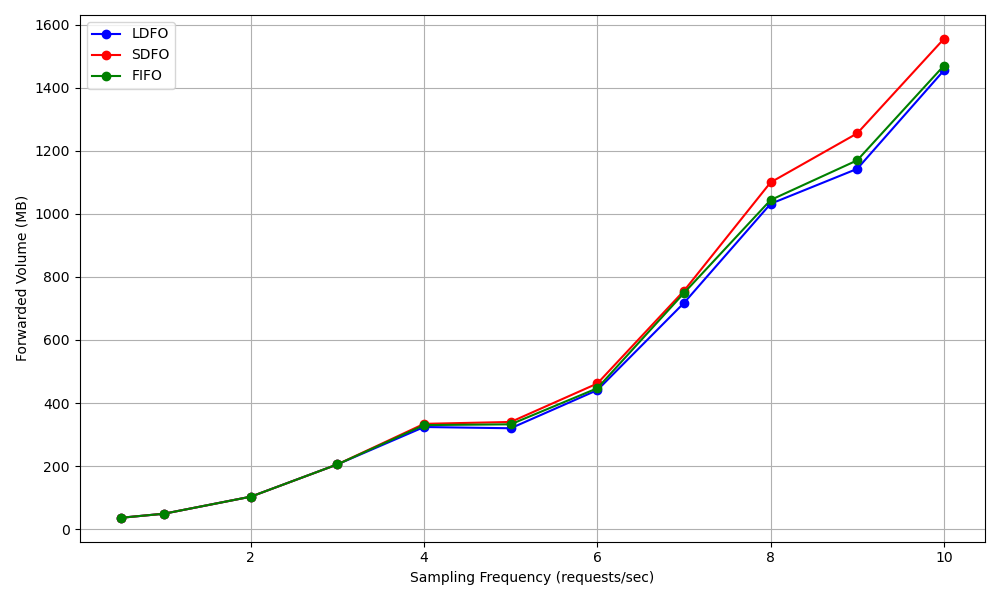
\includegraphics[width=\linewidth]{pics/expr/exp3_frequency_forwarded.png}
            \caption{跨节点协作总流量}
            \vspace{0.3cm}
        \end{subfigure}
        \begin{subfigure}{0.48\textwidth}
            \centering
            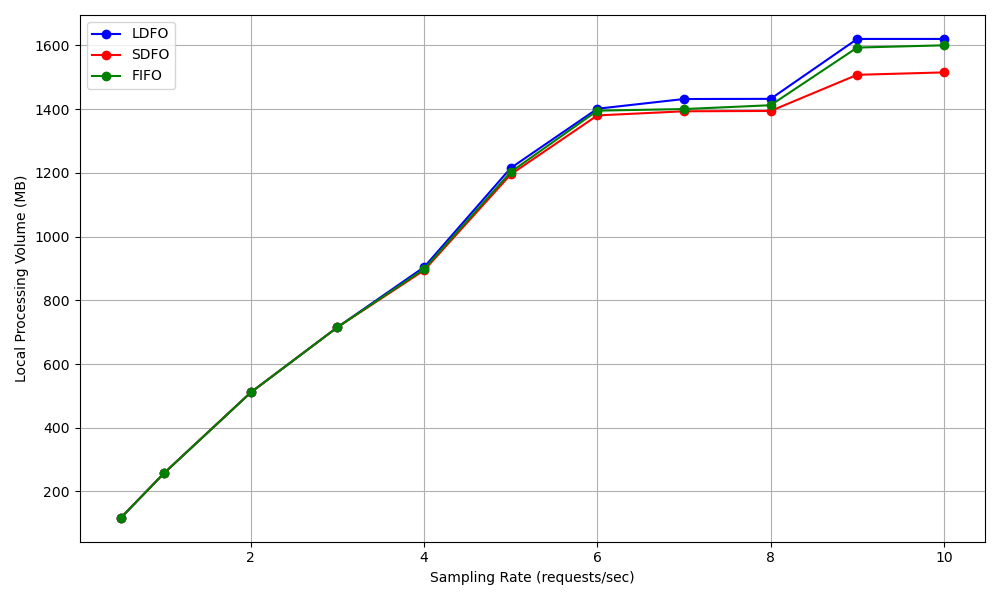
\includegraphics[width=\linewidth]{pics/expr/exp3_frequency_local_processed.png}
            \caption{本地处理的数据总流量}
            \vspace{0.3cm}
        \end{subfigure}
    \end{subfigure}
    \caption{不同优化策略下的本地调度性能对比}
    \label{fig:exp2}
\end{figure}

在边缘节点调度调度层次,本文重点比较了三种常见的队列优化策略:先进先出(First In First Out,FIFO)、最小数据量优先(Small Data First Out,SDFO)以及最大数据量优先(Large Data First Out,LDFO)。实验在相同的配置条件下进行,仅通过调整数据采集频率来观察三种优化策略的表现差异。如图 \ref{fig:exp2} 所示,实验结果表明,在边缘节点调度策略中,本文所用的LDFO 方式能够在保证本地设备数据流处理量的同时,有效减少跨节点协作流量,并最大化本地节点处理的数据总流量。这一策略显著提升了本地节点的资源利用率和整体调度效率,体现了其在高负载场景下的优越性。

\subsubsection{云端调度器实验分析}

\begin{figure}[ht]
  \centering
  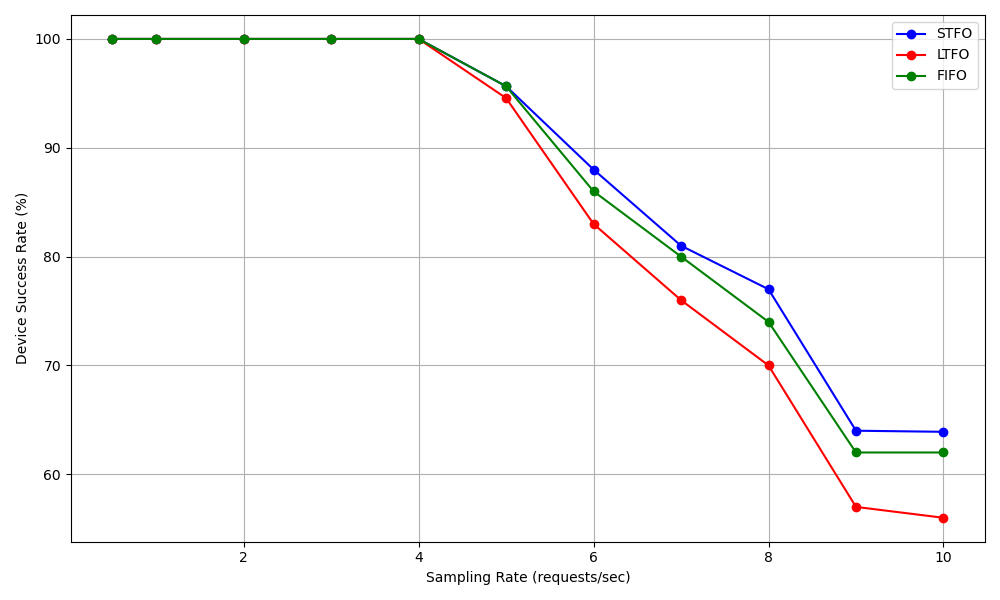
\includegraphics[width=0.8\linewidth]{pics/expr/exp5_frequency_device_success_rate.png}
  \caption{不同优化队列下的全局调度设备成功率}
  \label{fig:exp4}
\end{figure}

在云端调度层次,本文比较了三种常见的队列优化策略:最小任务优先(Small Task First Out, STFO)、最大任务优先(Large Task First Out, LTFO)以及先进先出(First In First Out,FIFO)。实验在相同的配置条件下进行,仅通过调整数据采集频率来观察三种队列的表现差异。由于本实验中云端资源是有限的,因此会出现任务失败的情况。如图 \ref{fig:exp4} 所示,实验结果表明,在云端全局调度策略中,本文所用的 STFO 方式能够显著提高设备的任务成功率。

\section{系统功能验证实验}

\subsection{模型推理实例动态部署功能验证}

为了验证模型推理实例动态部署功能的有效性,我们设计了一组实验,在多种架构的机器上利用 KEAS 实现目标监测模型的部署,并评估其运行准确性和适配能力。表\ref{tab:multi-arch-zhichi}展示了 KEAS 对四种主流架构的支持情况

\begin{table}[ht]
    \renewcommand{\arraystretch}{1.5}
    \centering
    \caption{KEAS对不同架构的机器的适配程度}
    \label{tab:multi-arch-zhichi}
    \begin{tabular}{|l|l|}
        \hline
        \textbf{架构类型} & \textbf{适配结果}  \\ \hline
        ARM32 (32-bit) & 支持 \\ \hline
        ARM64 (64-bit) & 支持 \\ \hline
        AMD64 & 支持 \\ \hline
        AMD64 (no-AVX2) & 支持 \\ \hline
    \end{tabular}
\end{table}

实验结果表明,KEAS 的部署模块能够成功支持在多种架构的机器上部署模型推理实例。在每个部署任务完成后,TensorFlow Serving 的运行日志关键部分均如图\ref{fig:aiapply}所示。这进一步验证了 KEAS 在主流硬件架构上的适配能力和稳定性。

\begin{figure}[ht]
    \centering
    \begin{lstlisting}[
        basicstyle=\small\ttfamily, 
        frame=single
    ]
[INFO] Successfully loaded servable version 
{name: yolov4-tiny version: 1}
[INFO] Running gRPC ModelServer at 0.0.0.0:8500 ...
[INFO] Exporting HTTP/REST API at:localhost:8501 ...
\end{lstlisting}
    \caption{目标监测模型在 TensorFlow Serving 上的运行日志}
    \label{fig:aiapply}
\end{figure}

此外,我们还测试了不同深度学习框架之间的模型转换功能,并基于 YOLO 模型验证了其可行性。具体而言,实现了从 PyTorch、Keras 和 ONNX 到 TensorFlow 模型的转换,确保这些模型能够在 KEAS 系统中无缝集成和部署。表~\ref{tab:model-conversion-results} 展示了不同框架间模型转换的验证结果。

\begin{table}[ht]
    \renewcommand{\arraystretch}{1.5}
    \centering
    \caption{不同框架间模型转换的验证结果}
    \label{tab:model-conversion-results}
    \begin{tabular}{|l|l|l|}
        \hline
        \textbf{源框架} & \textbf{目标框架} & \textbf{转换结果} \\ \hline
        PyTorch & TensorFlow & 支持 \\ \hline
        Keras & TensorFlow & 支持 \\ \hline
        ONNX & TensorFlow & 支持 \\ \hline
    \end{tabular}
\end{table}


\subsection{模型推理实例批处理功能验证}

为验证模型推理实例批处理测试功能的有效性,并快速确定模型的最优批处理大小,同时为之前的仿真实验提供真实数据支撑,本文在系统运行过程中采集了批处理测试的相关数据,并分别测试了模型推理实例在 CPU 和 GPU 环境下的运行性能,以下给出 YOLOv4 模型的相关采集数据。

\begin{figure}[ht]
  \centering
  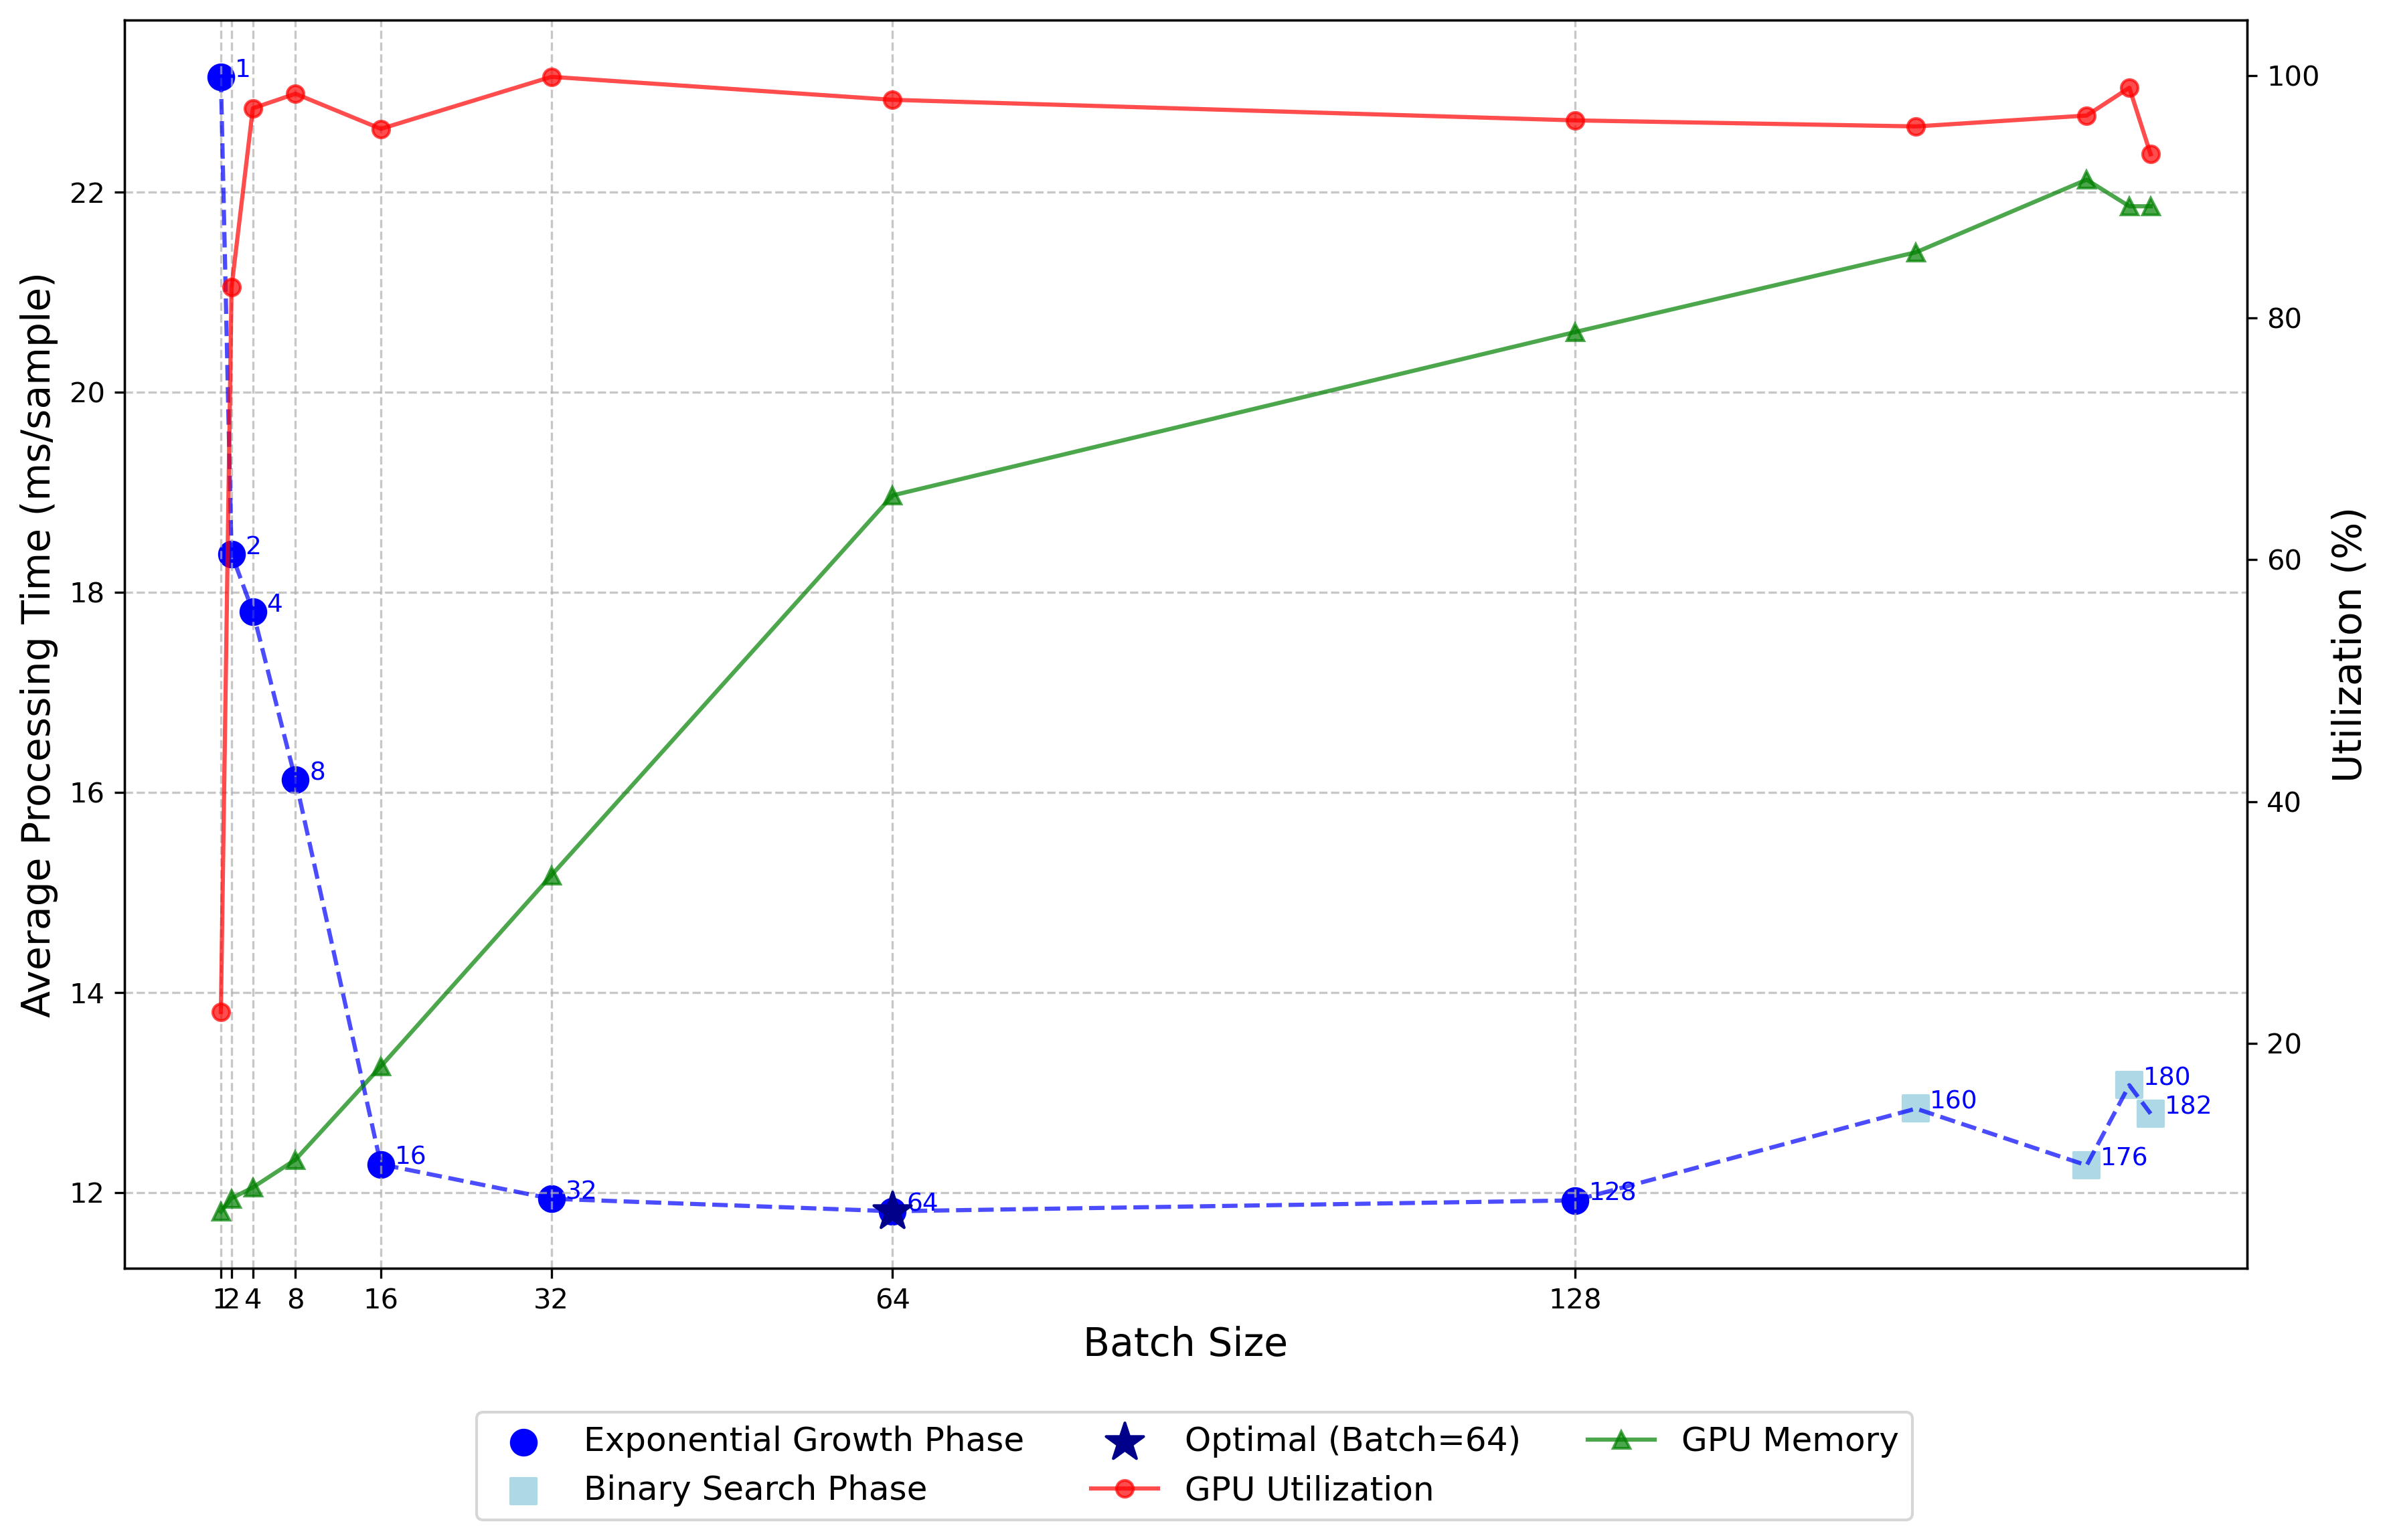
\includegraphics[width=0.8\linewidth]{pics/expr/yolov3_gpu_performance.png}
  \caption{GPU上的目标监测模型批处理性能分析}
  \label{fig:expaigpu}
\end{figure}

如图 \ref{fig:expaigpu} 所示,在 GPU 环境下运行 YOLOv4 相关模型时,随着批处理大小的增加,GPU 的利用率和显存占用呈现逐步上升的趋势。批处理规模的扩大使得更多的数据能够被并行加载到显存中进行计算,从而显著提高了 GPU 的计算资源利用率。然而,由于 GPU 显存容量的限制,当批处理大小达到一定阈值时,显存占用接近硬件上限,并最终因显存不足(Out of Memory, OOM)而无法继续扩展批处理规模。实验结果表明,在该显卡配置下,YOLO 模型在稳定运行状态下平均处理一张图片所需时间为 11.8 毫秒。

\begin{figure}[ht]
  \centering
  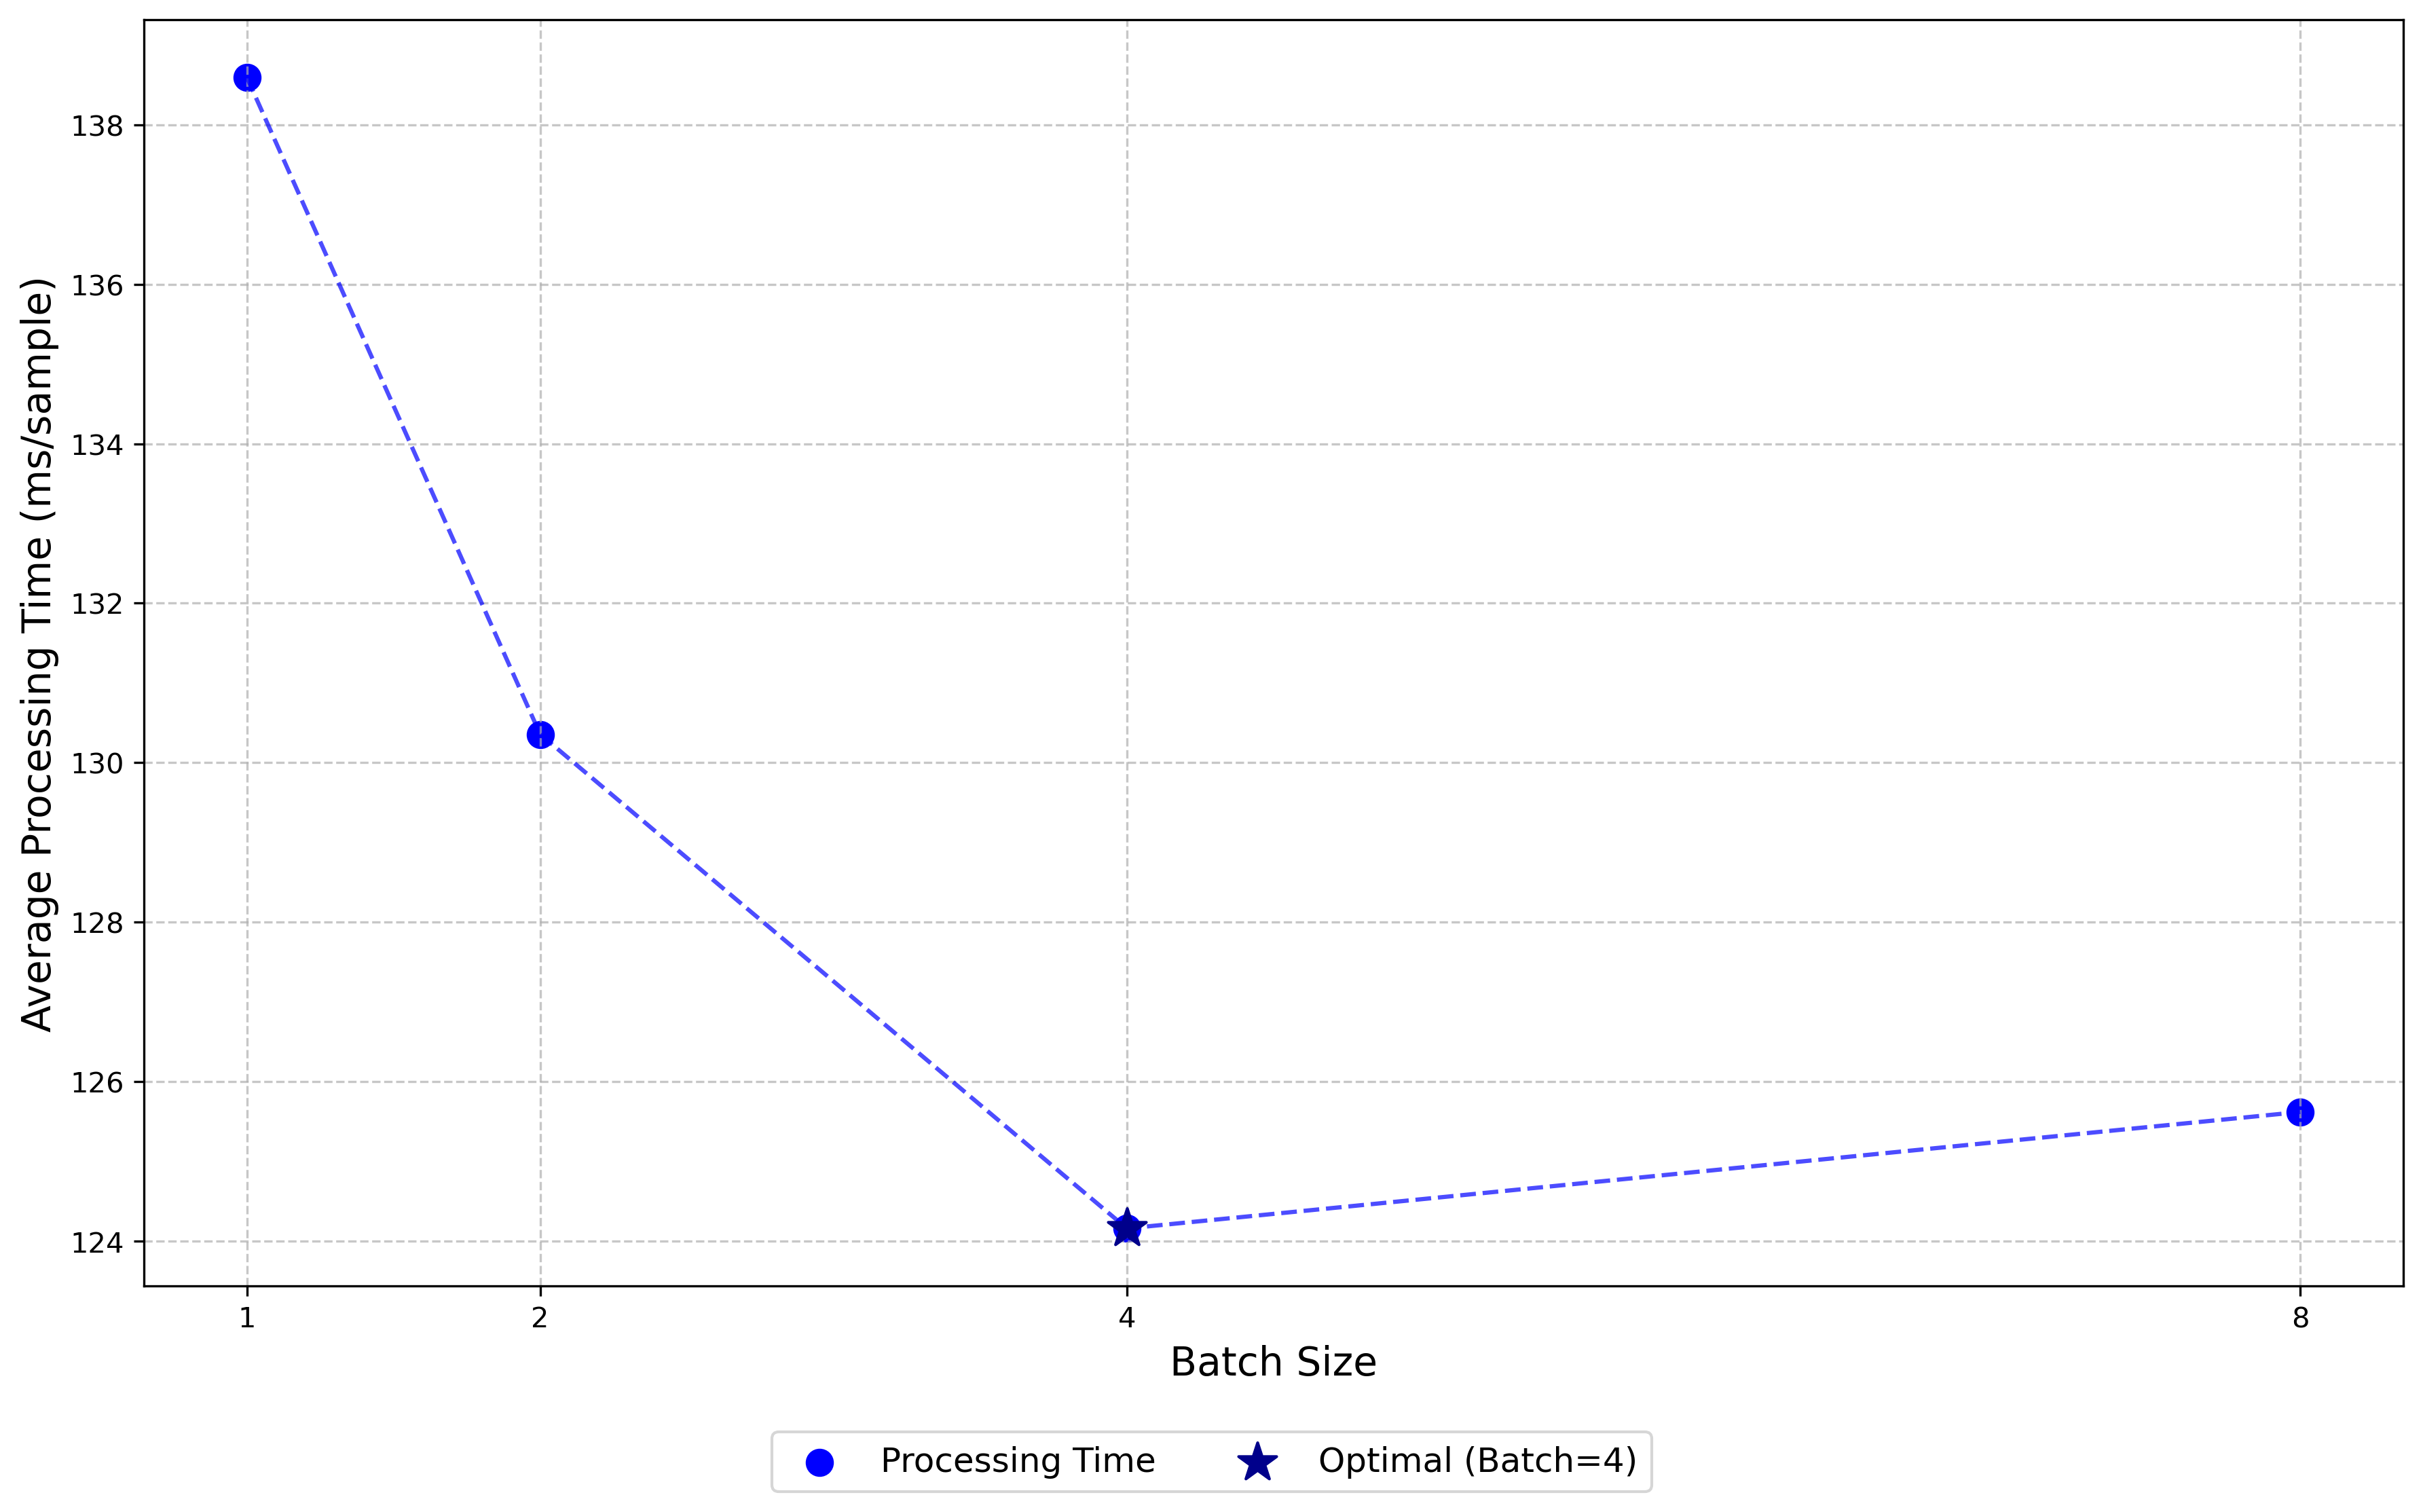
\includegraphics[width=0.8\linewidth]{pics/expr/yolov3_cpu_performance.png}
  \caption{CPU上的目标监测模型批处理性能分析}
  \label{fig:expaicpu}
\end{figure}

与GPU的众核架构不同,CPU的核心数量有限,且缺乏针对大规模数据并行计算的硬件优化,这使得通过批处理提升计算吞吐量的效果存在显著差异。如图 \ref{fig:expaicpu} 所示,在 CPU 环境下采用批处理策略时,由于无法充分发挥线程级并行优势,当单次批处理规模超过物理核心数量后性能提升幅度迅速收敛,此时搜索算法在性能提升不显著的情况下会迅速停止搜索。实际测试数据显示,该 CPU 配置下处理单张图片耗时达到 124 毫秒。

\subsection{系统监控服务功能验证}

本系统监控服务主要由探针模块和汇总模块两部分组成。探针模块采用主被动结合的混合监测方案,通过网络探针实时检测网络状态;同时,模型推理服务模块会持续监控其运行速度,并将采集到的相关数据上传至边缘集群。汇总模块负责对这些数据进行处理,为集群级别的资源调度与负载均衡提供重要依据。随后,边缘集群进一步汇总这些数据并将其上传至云端,从而支持全局范围内的资源调度与优化。汇总的数据存储在 Prometheus 中,并基于预定义的 Grafana 模板生成系统监控仪表盘。通过实验验证,我们可以在仪表盘中查看各个节点的详细监测数据,如图\ref{fig:grafana}所示。

\begin{figure}[ht]
  \centering
  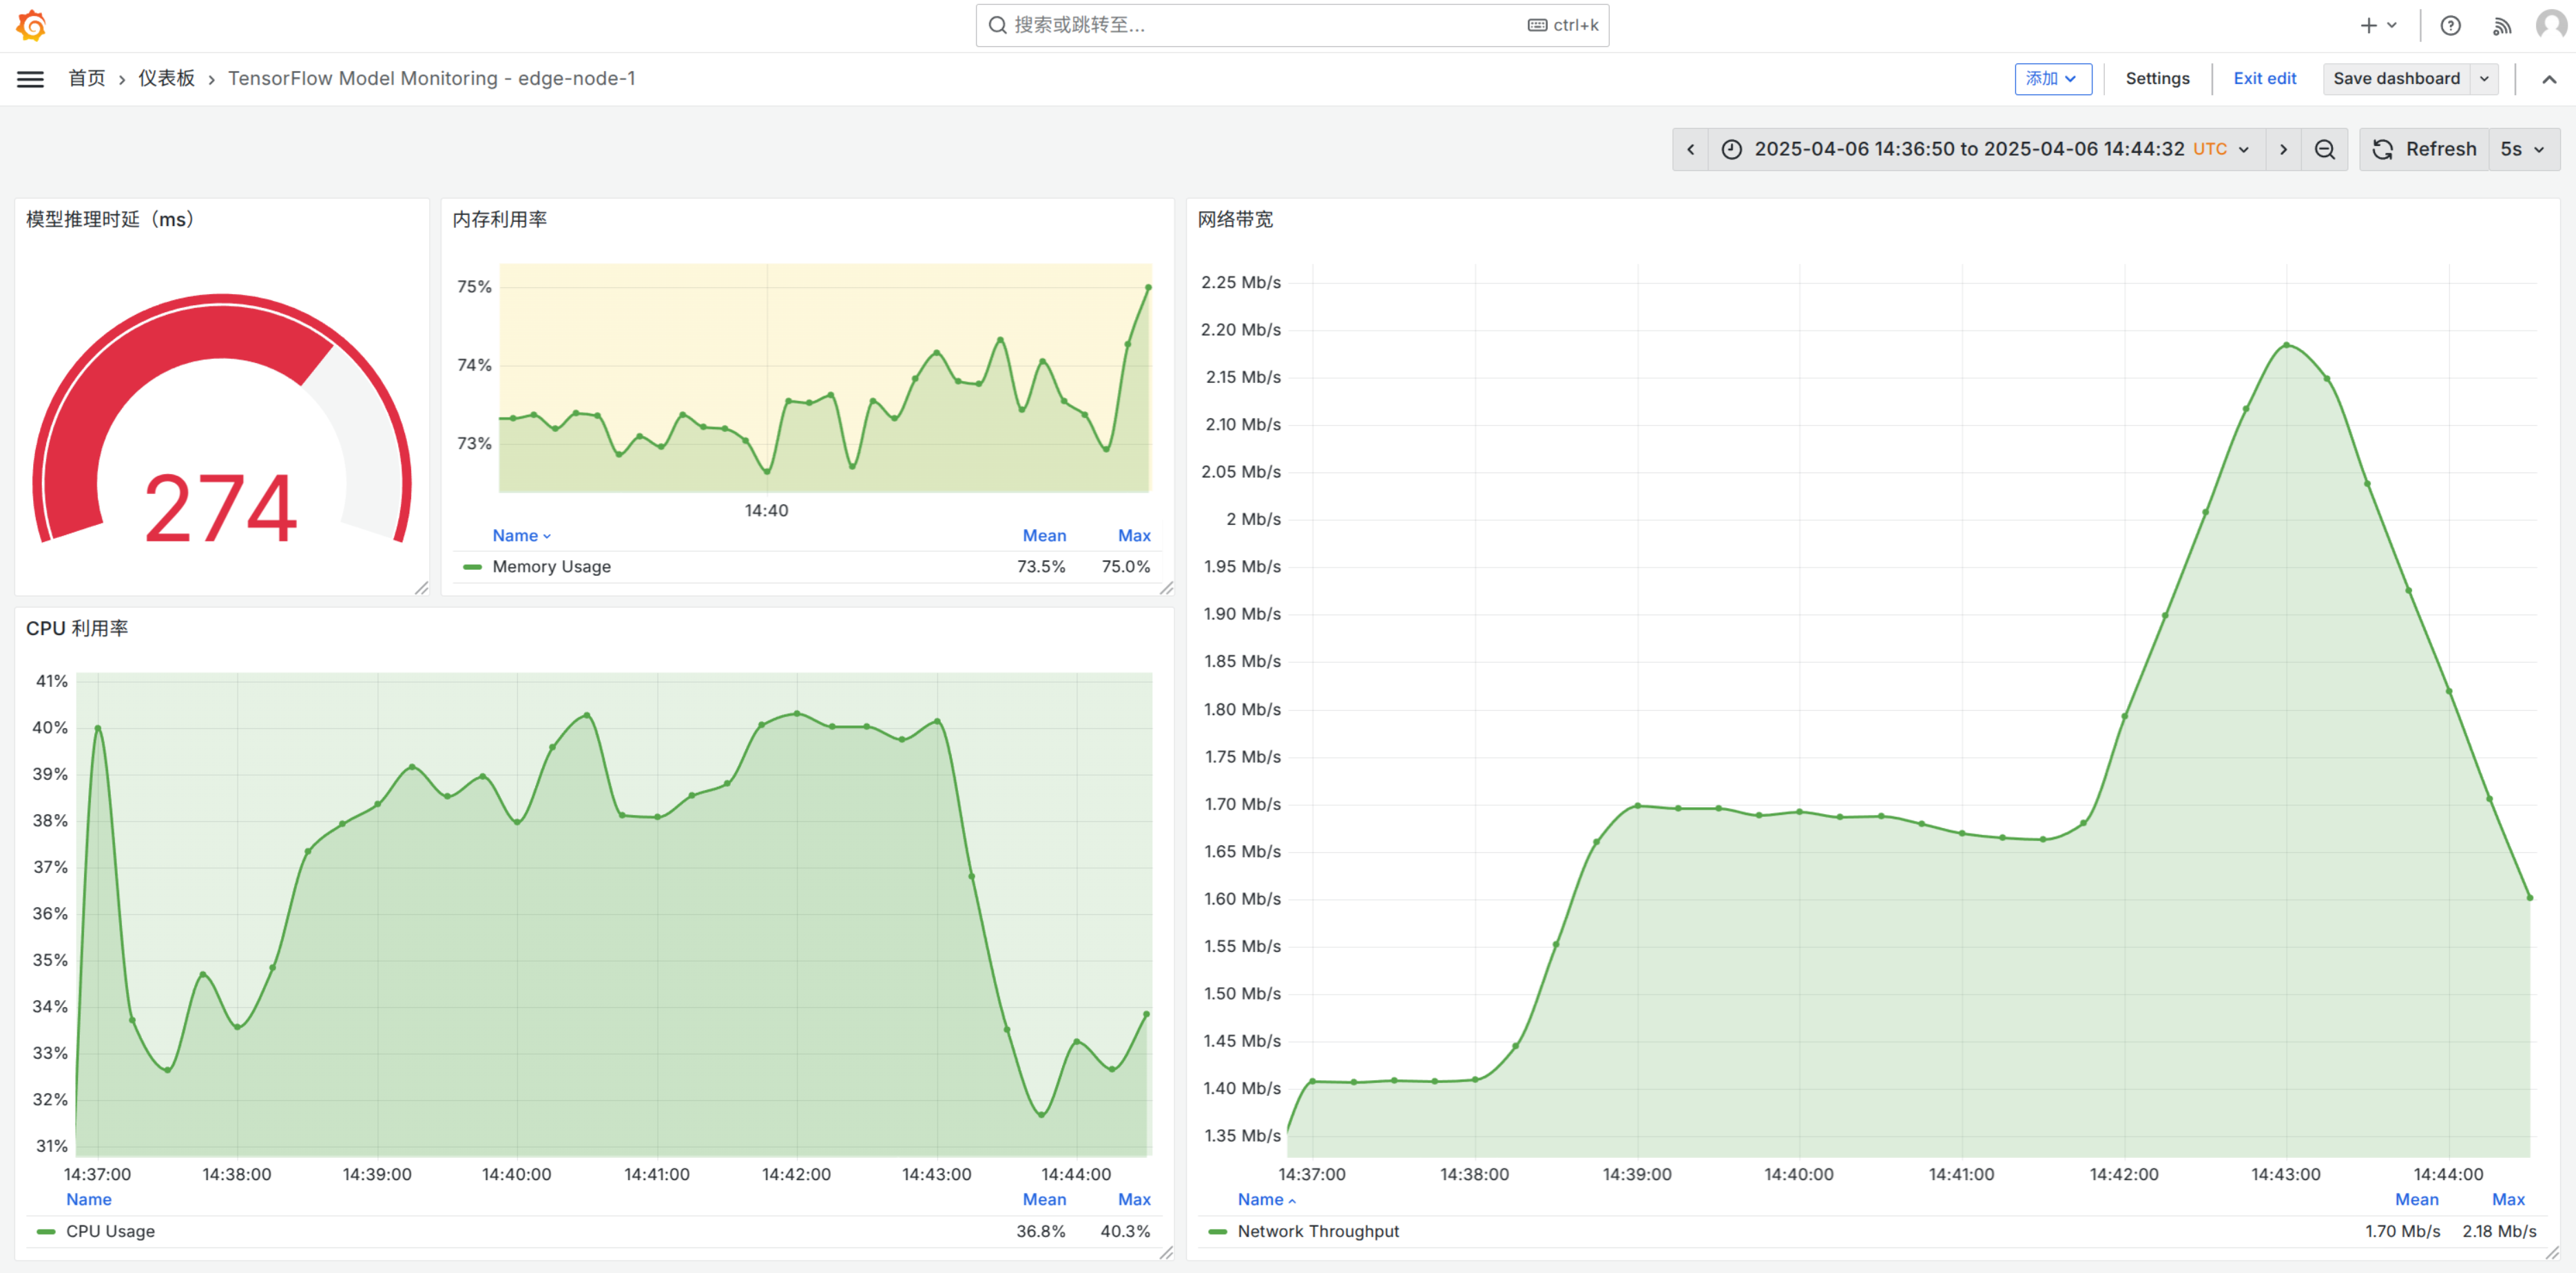
\includegraphics[width=\linewidth]{pics/expr/5-6grafana.png}
  \caption{Grafana 监控仪表盘界面}
  \label{fig:grafana}
\end{figure}

\section{系统性能评估实验}

为了精确衡量调度器的性能,本文在实验中采用了时间戳追踪法。具体而言,在请求生成路由时立即记录第一个时间戳作为等待时间的起点;当系统成功匹配到合适节点并将该请求纳入处理队列时,记录第二个时间戳以标记实际处理开始的时间点;最后,在请求完成全部处理流程后记录第三个时间戳。通过这种方式,可以直接计算出请求在队列中的等待时间和节点实际处理请求所需的时间。

\begin{table}[ht]
    \renewcommand{\arraystretch}{1.5}
    \centering
    \caption{调度器性能评估实验数据}
    \label{tab:performance}
    \begin{tabular}{lll}
        \toprule
        \textbf{平均响应时间} & \textbf{平均等待时间} \\
        \midrule
        $247.29 \, \text{ms}$ & $126.88 \, \text{ms}$  \\ 
        \bottomrule
    \end{tabular}
\end{table}

在上述实验设置下,本文获取了表 \ref{tab:performance} 中的数据,展示了调度器的平均响应时间和平均等待时间。结果显示,调度器表现出较高的处理效率和较低的等待时间,表明其具有良好的性能表现。

\section{本章小结}

本章对 KEAS 方案进行全面实验评估,分为核心算法仿真、系统功能验证和性能评估三部分。核心算法仿真实验通过模拟云边环境中的计算节点与设备流式数据生成过程,验证分层调度优化算法在服务质量指标(如调度成功率)上的表现。系统功能验证实验测试各核心模块的功能完整性,确保其稳定运行与协同能力。系统性能评估实验深入分析了分层调度决策对响应时间的影响。
